

\section{Cơ sở lý thuyết về Thị giác Máy tính}

\subsection{Định nghĩa và mục tiêu}
Thị giác Máy tính (Computer Vision, CV) là lĩnh vực trí tuệ nhân tạo cho phép máy tính thu nhận, xử lý, phân tích và diễn giải hình ảnh hoặc video nhằm đạt được khả năng “hiểu” nội dung ở cấp độ cao. Mục tiêu chính là mô phỏng khả năng thị giác của con người với tốc độ và quy mô vượt trội.

\subsection{Pipeline cơ bản của hệ thống CV}
Một hệ thống CV điển hình gồm các bước sau:

\begin{enumerate}
    \item \textbf{Thu nhận dữ liệu}: Hình ảnh hoặc video từ cảm biến camera.
    \item \textbf{Tiền xử lý}: Chuẩn hóa kích thước, điều chỉnh độ sáng/tương phản, loại bỏ nhiễu.
    \item \textbf{Trích xuất đặc trưng}: Biểu diễn hình ảnh ở dạng trừu tượng để mô hình học máy có thể xử lý hiệu quả.
    \item \textbf{Phân tích và ra quyết định}: Phân loại, nhận dạng đối tượng, phát hiện biên hoặc phân đoạn ảnh dựa trên các đặc trưng đã trích xuất.
\end{enumerate}

\begin{figure}[h]
    \centering
    
\includegraphics[width=0.9\textwidth]{vision_flow.png}
    \caption{Quy trình tổng thể của một hệ thống Thị giác Máy tính từ ảnh đầu vào đến kết quả phân tích.}
    \label{fig:cv_pipeline}
\end{figure}

\subsection{Các mô hình cốt lõi trong CV hiện đại}
\subsubsection{Mạng nơ-ron tích chập (CNN)}
CNN là kiến trúc mạng nơ-ron phổ biến để xử lý dữ liệu hình ảnh, sử dụng các lớp tích chập và gộp (pooling) để học các đặc trưng phân cấp.

\begin{itemize}
    \item \textbf{Phép tích chập (Convolution)}: Trích xuất đặc trưng từ hình ảnh đầu vào bằng cách áp dụng bộ lọc (kernel) $K$ lên ảnh $I$:
    \begin{equation}
    (I * K)(i, j) = \sum_{m} \sum_{n} I(i-m, j-n) K(m, n)
    \end{equation}

    \item \textbf{Phép gộp (Pooling)}: Giảm kích thước không gian và tăng khả năng trừu tượng. Ví dụ, max pooling trên cửa sổ $2 \times 2$:
    \begin{equation}
    O_{i,j} = \max \left( I_{2i, 2j}, I_{2i+1, 2j}, I_{2i, 2j+1}, I_{2i+1, 2j+1} \right)
    \end{equation}
\end{itemize}

\begin{figure}[h]
    \centering
    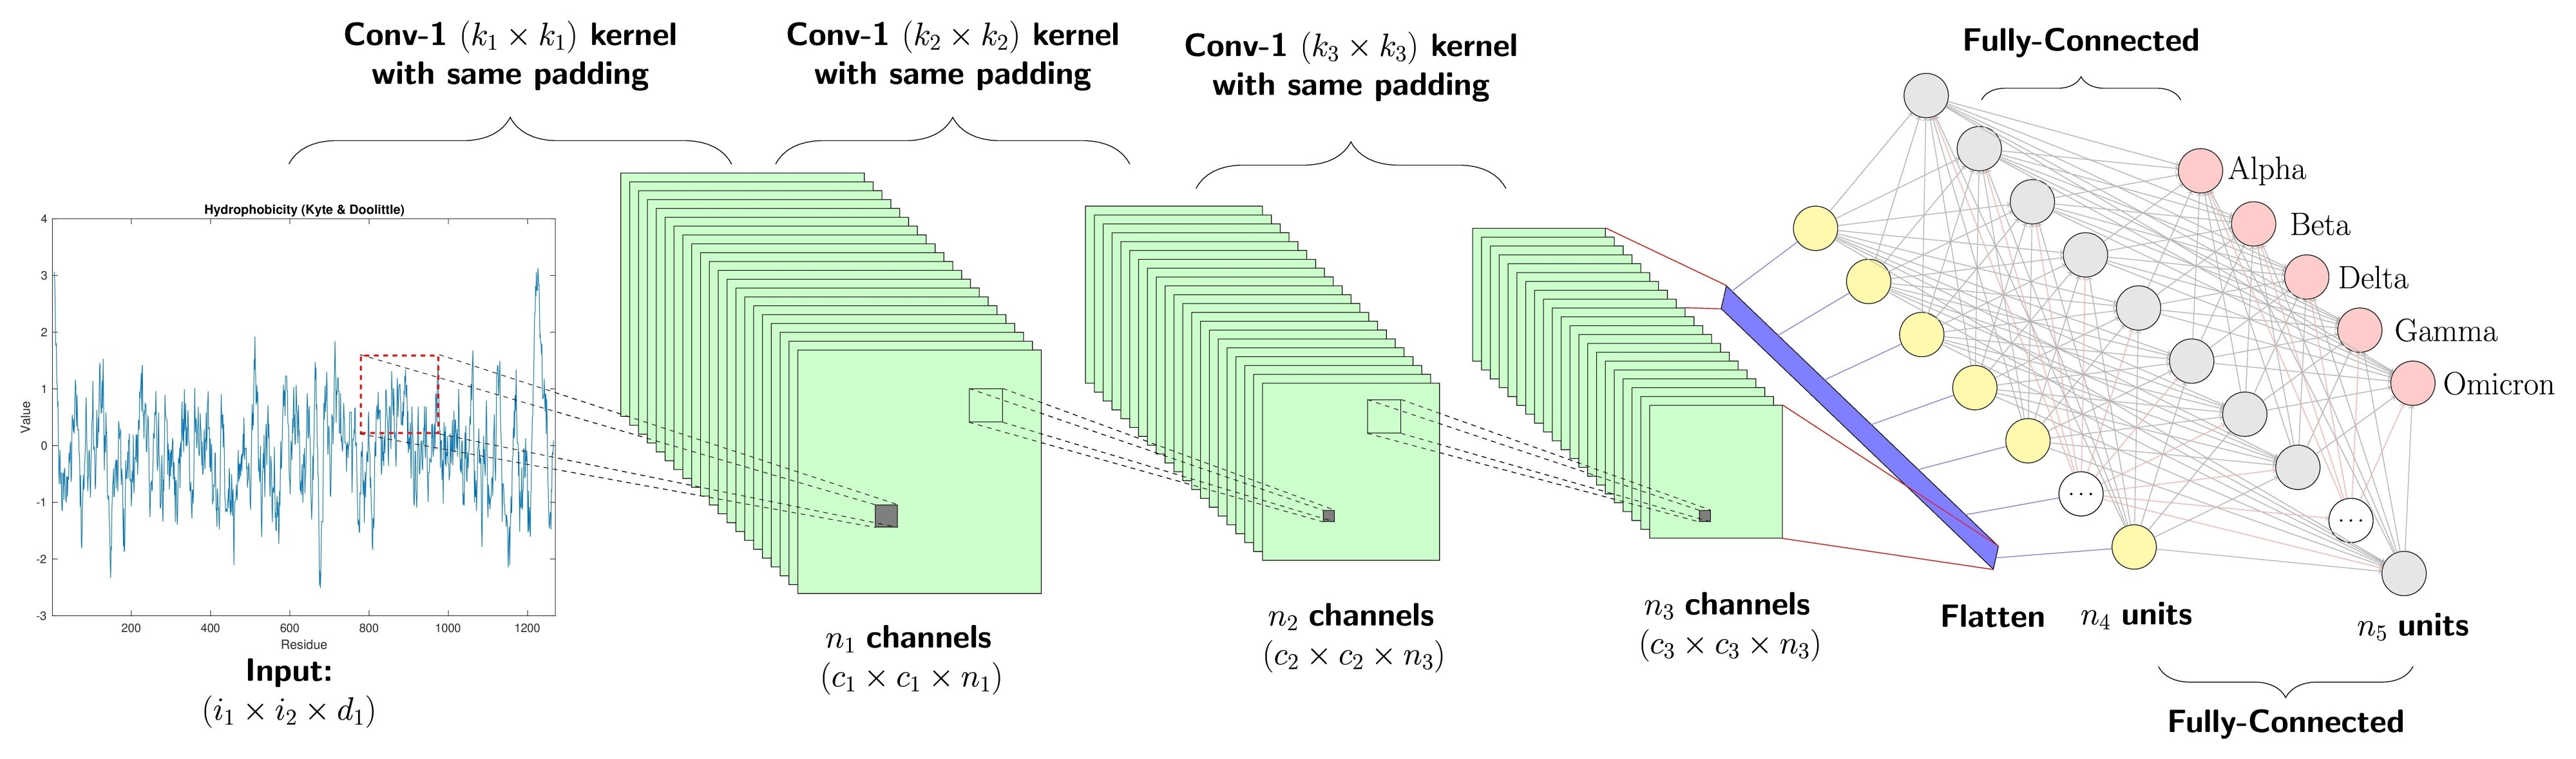
\includegraphics[width=0.8\textwidth]{2_2_convolution.jpeg}
    \caption{Minh họa các phép toán tích chập và gộp.}
    \label{fig:cnn_ops}
\end{figure}

Các kiến trúc CNN nổi bật: \textbf{ResNet} \cite{he2016deep}, \textbf{Faster R-CNN} \cite{ren2015faster}, \textbf{YOLO} \cite{redmon2016you}.  

\subsubsection{Mô hình dựa trên Transformer}
Transformer, đặc biệt là Vision Transformer (ViT) \cite{dosovitskiy2021image}, chia hình ảnh thành các miếng vá (patches) và xử lý chúng như chuỗi token, sử dụng cơ chế tự chú ý (self-attention) để học mối quan hệ giữa các vùng ảnh:
\begin{equation}
\text{Attention}(Q, K, V) = \text{softmax}\left(\frac{QK^T}{\sqrt{d_k}}\right)V
\end{equation}

\begin{figure}[h]
    \centering
    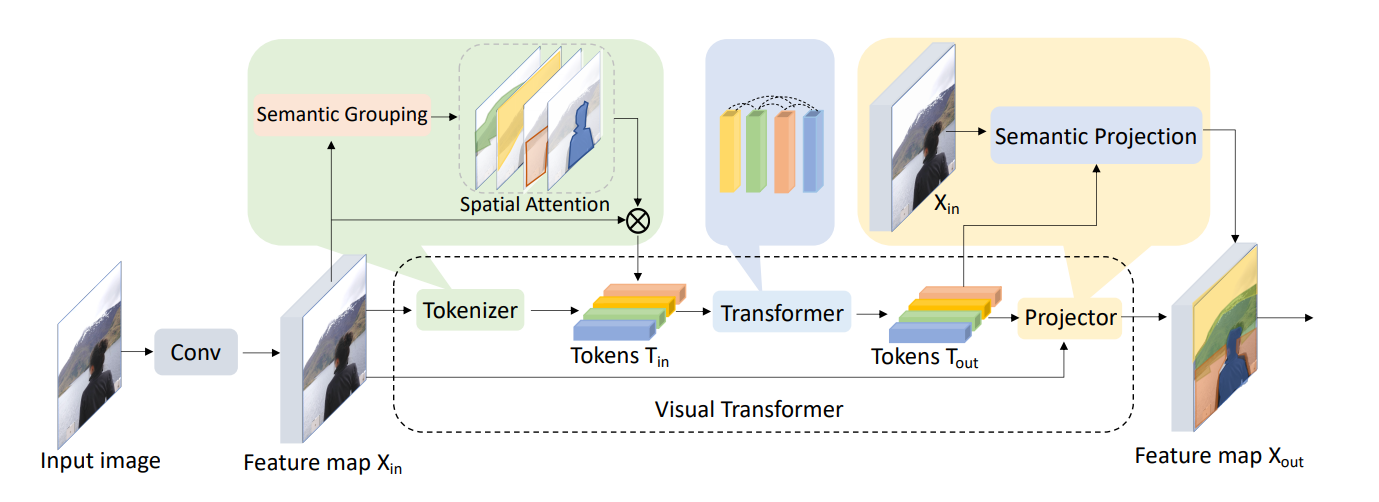
\includegraphics[width=0.9\textwidth]{visual_transformer.png}
    \caption{Kiến trúc Vision Transformer (ViT).}
    \label{fig:vit_arch}
\end{figure}

\subsection{Tập dữ liệu và metrics đánh giá}
Để đánh giá hiệu quả mô hình CV, sử dụng các tập dữ liệu và metrics chuẩn:

\begin{itemize}
    \item \textbf{Tập dữ liệu}: ImageNet \cite{deng2009imagenet}, COCO \cite{lin2014microsoft}, Pascal VOC \cite{everingham2015pascal}, Cityscapes \cite{cordts2016cityscapes}.
    \item \textbf{Metrics}: 
    \begin{itemize}
        \item \textbf{IoU (Intersection over Union)}: Độ trùng khớp giữa dự đoán và ground truth.
        \item \textbf{mAP (Mean Average Precision)}: Tiêu chuẩn cho bài toán phát hiện đối tượng.
        \item \textbf{F1-score}: Trung bình điều hòa giữa precision và recall, phổ biến trong bài toán phân loại.
    \end{itemize}
\end{itemize}

\subsection{Tóm tắt}
Phần này cung cấp kiến thức nền tảng về CV, bao gồm pipeline, các mô hình học sâu cốt lõi và cách đánh giá hiệu suất. Những kiến thức này sẽ được tham chiếu trực tiếp trong phần HPE và MediaPipe trong chương tiếp theo.
